\section{Discussion} \label{sec:disc}



In general, lower medians and overall distribution of cost values obtained by XQAOA$_1^\text{X=Y}$ compared to QAOA$_1$ and MAQAOA$_1$ indicates that XQAOA$_1^\text{X=Y}$ is more likely to find better solutions for any random set of initial parameter values. As was the purpose of introducing the additional products in the mixing Hamiltonian, it is likely that the comparative performance of XQAOA$_1^\text{X=Y}$ is due to different trajectories traced through the Hilbert solution space, attributed to the Pauli-$Y$ gates governed by the variational parameter $\pmb{\alpha}$. \citet{vijendran2023expressive} also reported similar findings, however, the XQAOA$_1^\text{X=Y}$ outperformed all algorithms and was on par with the Gurobi optimser. Indeed, their analysis was on $D$-regular graphs with 128 and 256 vertices ($3\leq D\leq 10$) which are comparatively sparser graph instances than the ones analysed in this project, so our XQAOA$_1^\text{X=Y}$ performance may be attributed to the dependence of relatively more variational parameters.

We present the dataset for fixed $m=8$ on a linear scale in Figure \ref{fig:fixed_m_normal} for ease of visualisation (visualisation for the dataset for fixed $n=10$ is not as informative on a linear scale since the medians increase exponentially with the problem ratio). From the performance max-cut algorithms QAOA$_1$, MAQAOA$_1$, XQAOA$_1^\text{X=Y}$, and Goemans-Williamson on the dataset for fixed $m=8$, the problem ratio was not a good indicator of the ``hardness'' of a given partitioning problem. Indeed, this could be due to the nature of transforming an NPP into a complete graph and solving a max-cut problem - the hardness indicated by the problem ratio simply does not translate. Gurobi was benchmarked by minimising the cost function of NPP so it exhibits similar trends to the classical heuristics. 


\begin{widetext}

\begin{minipage}{\linewidth}

\begin{figure}[H]
\captionsetup{justification=centering}
    \centering
    \begin{subfigure}[b]{\textwidth}
        \centering
        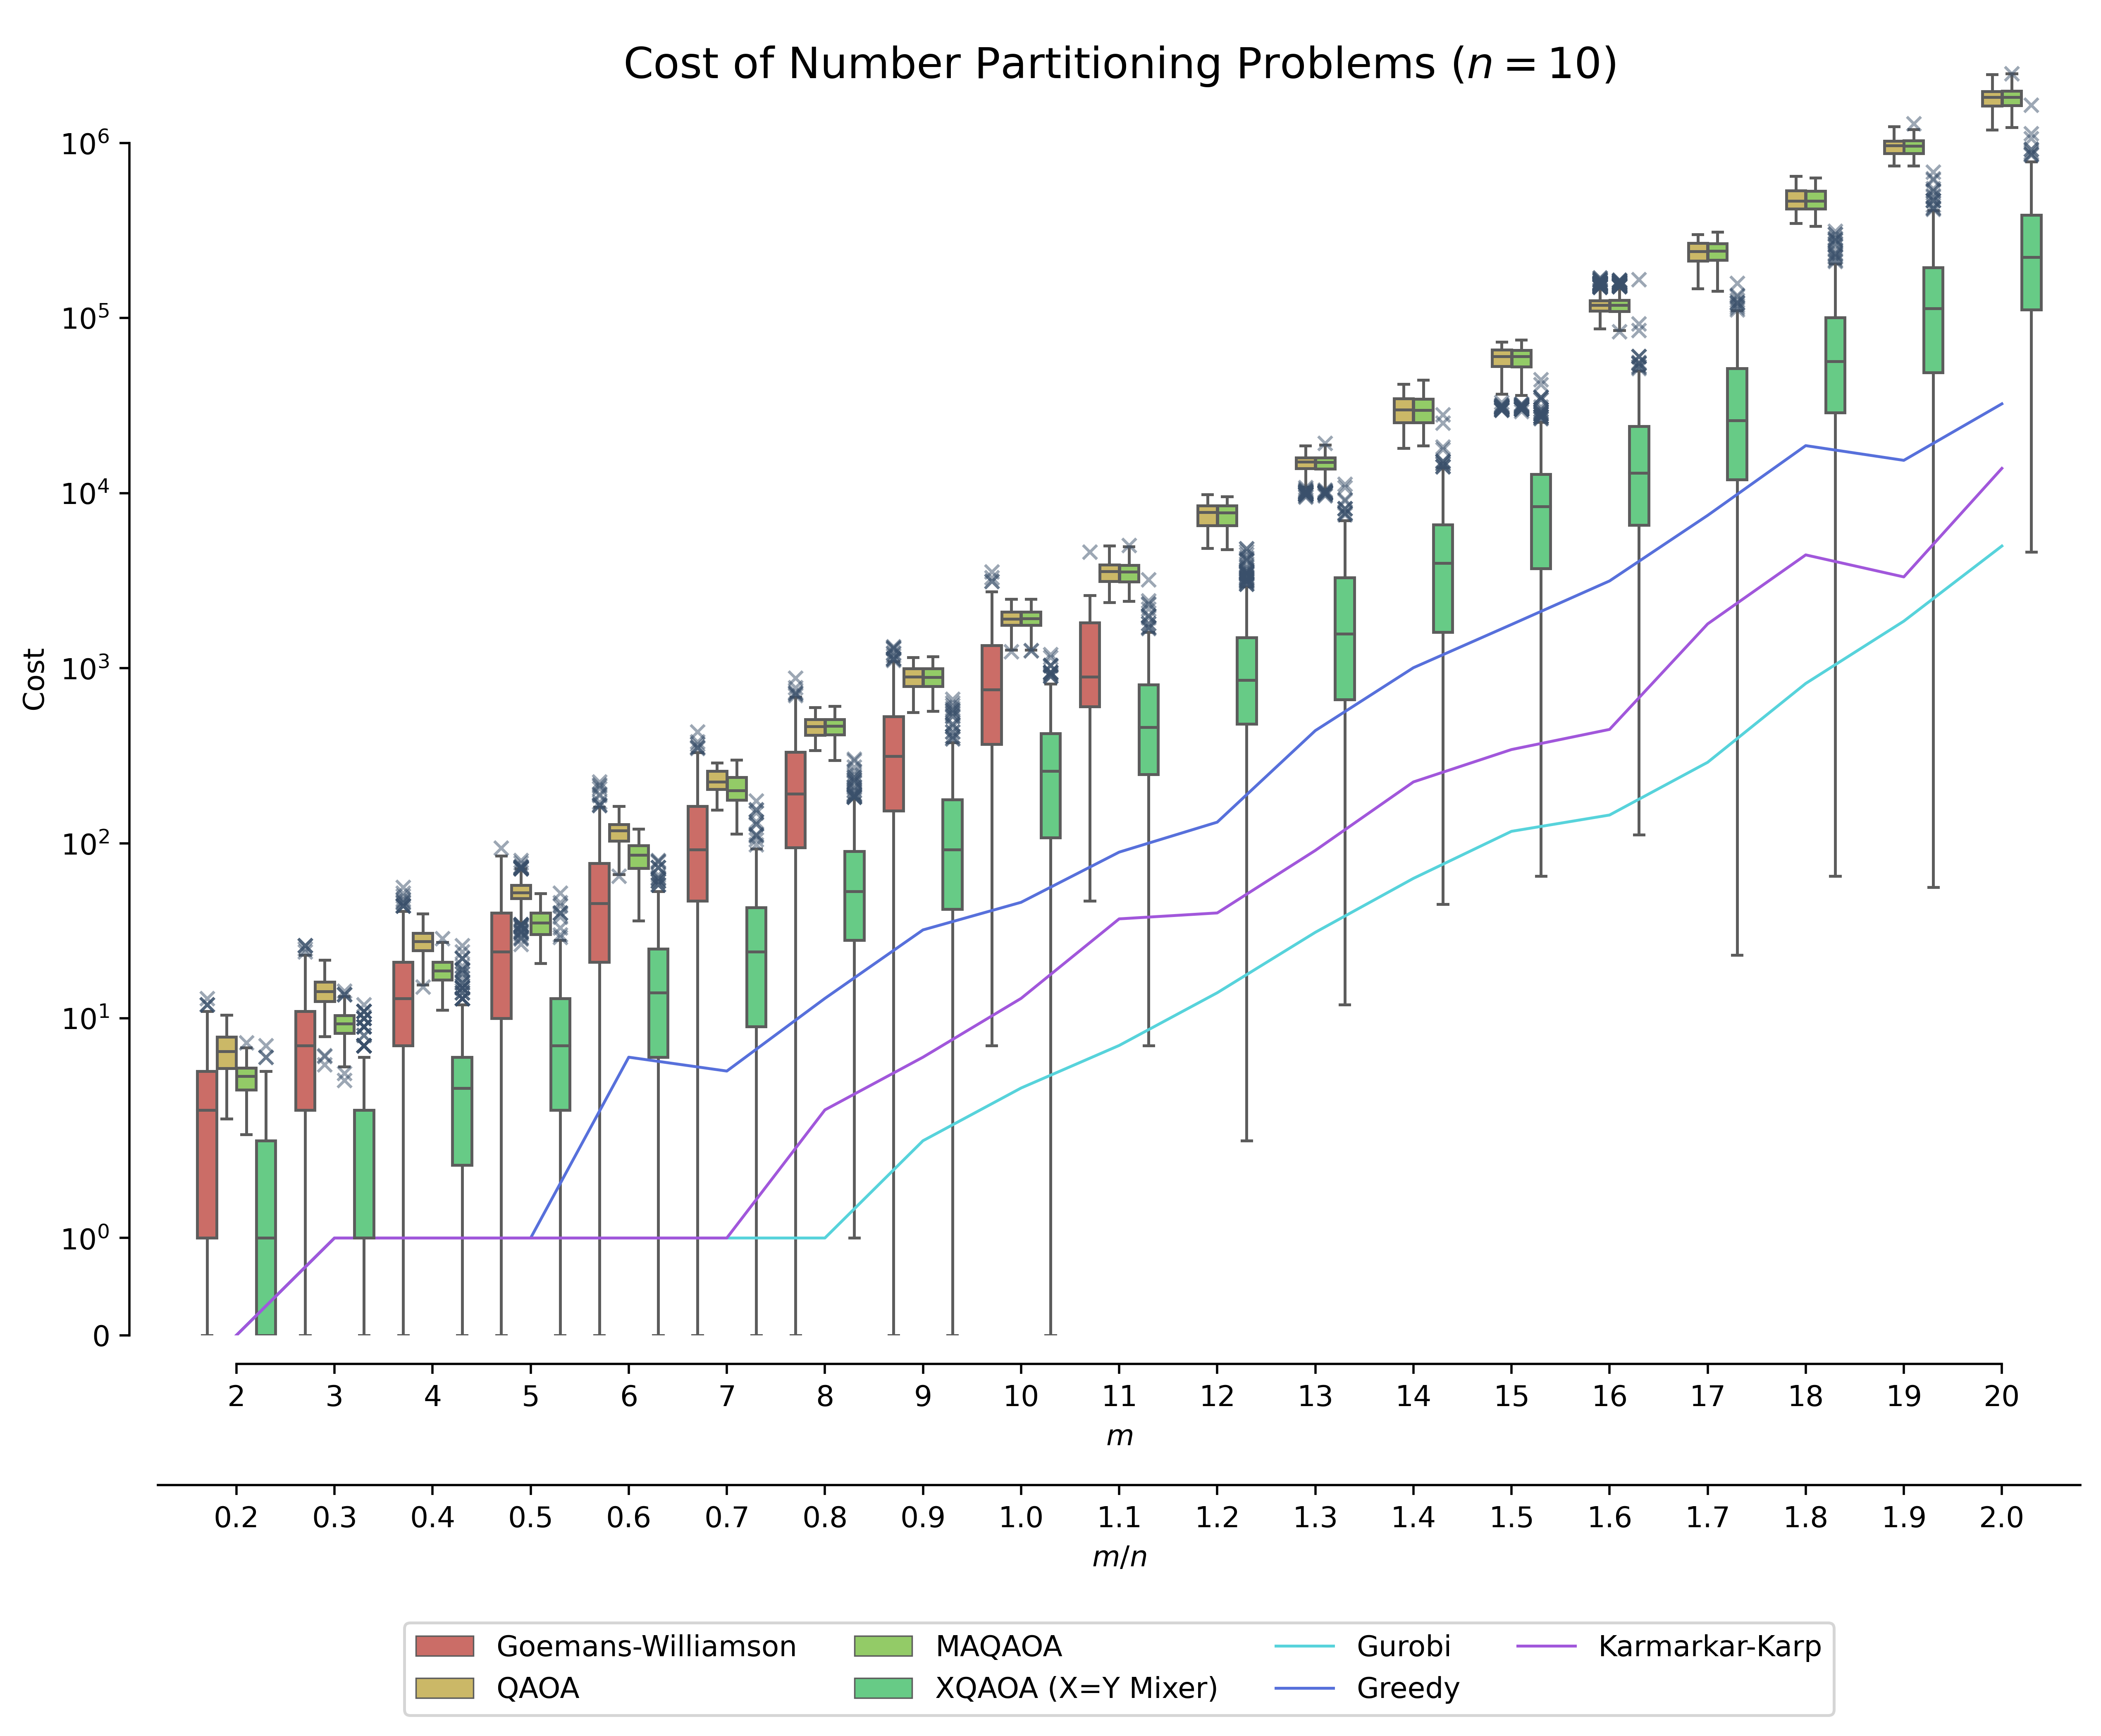
\includegraphics[scale=0.55]{"../figures/fixed_n.png"}
        \caption{Dataset for problem ratios with fixed $n=10$.}
        \label{fig:fixed_n}
    \end{subfigure}

    \hfill

    \begin{subfigure}{\textwidth}
        \centering
        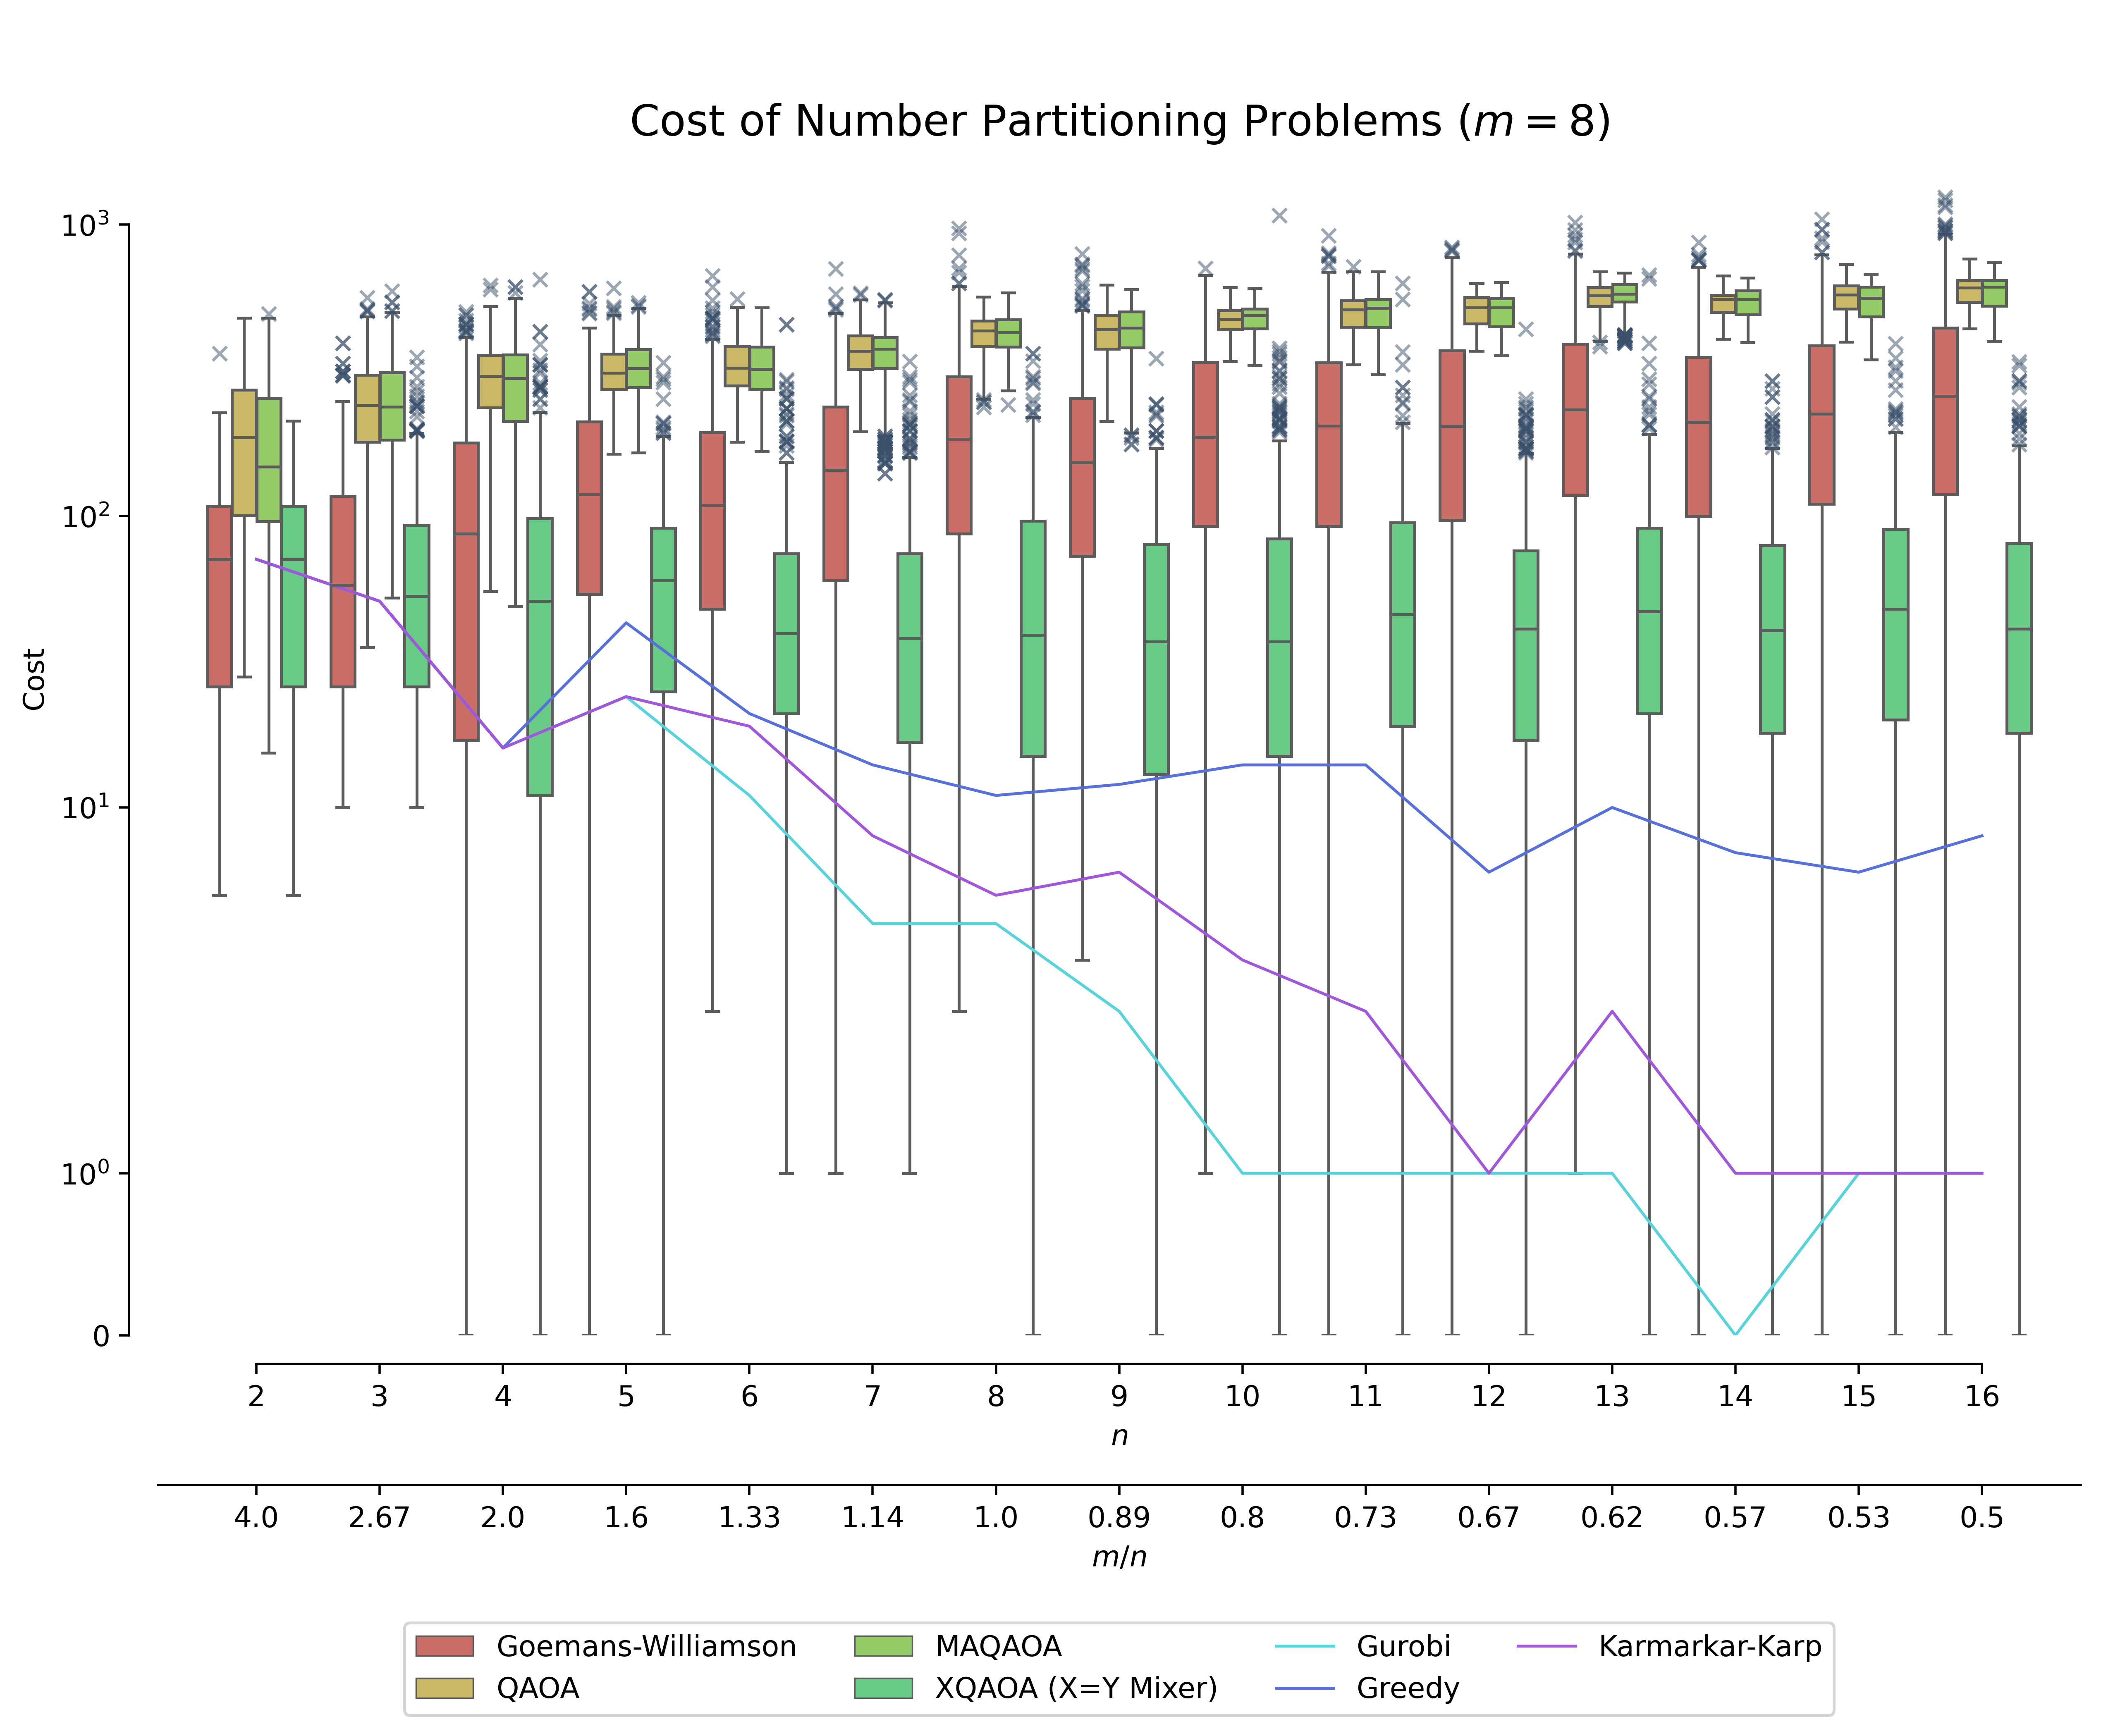
\includegraphics[scale=0.55]{"../figures/fixed_m.png"}
        \caption{Dataset for problem ratios with fixed $m=8$.}
        \label{fig:fixed_m}
    \end{subfigure}
    \caption{Box plot and line plot comparing average set-difference found by analytic forms of quantum algorithms for depth $p=1$ and classical algorithms for problem ratios $m/n$. The algorithms were benchmarked against the set-difference found by the classical optimiser Gurobi. For each problem ratio, 25 random problem instances were generated. The data used to create the box plot comes from 20 random cuts generated using the Goemans-Williamson algorithm, and 20 random initialisations of variational parameters for QAOA and its variants for each problem instance. The crosses represent outliers. The line plot for Gurobi, greedy and Karmarkar-Karp represents the median cost found across all 25 problems for each problem ratio.}
    
\end{figure}
\end{minipage}
\end{widetext}
%

\subsection{Ansatz Considerations} \label{disc:ansatz}
One of the biggest challenges in using VQA's such as QAOA is the issue of barren plateaus which refers to the phenomenon where the gradients of the objective function become exponentially vanshing with system size \cite{mcclean2018barren}, making it difficult to find the optimal solution using gradient-based optimisation methods. Because the ansatz is problem-specific, one needs to explore an exponentially large space to find a solution, and so, with random initialisations of variational parameters, the probability of finding the solution is exponentially small. If the initial point is near a local optimum or resides on a barren plateau, gradient-based optimisers will converge on a local optima. We see that QAOA$_1$, MAQAOA$_1$, and XQAOA$_1^\text{X=Y}$ return a wide range of approximate solutions for the same problem, however, with the right choice of parameters, XQAOA$_1^\text{X=Y}$ can often achieve a perfect or near-perfect cut on par with the Gurobi optimiser. 

We also note the large spread of distributions attained by the Goemans-Williamson algorithm. Although Goemans-Williamson achieves an approximation ratio of 0.878 in the worst case at the asymptotic limit \cite{goemans1994879}, randomly vectors are generated to perform its hyperplane rounding. This means that problem instances can vary significantly, resulting in distributions that increase in spread as $n$ and $m$ grows. To find better approximations using Goemans-Williamson, the precision (i.e., repetitions for a problem instance) would need to increase exponentially with the size of the problem.
\begin{figure}
    \centering
    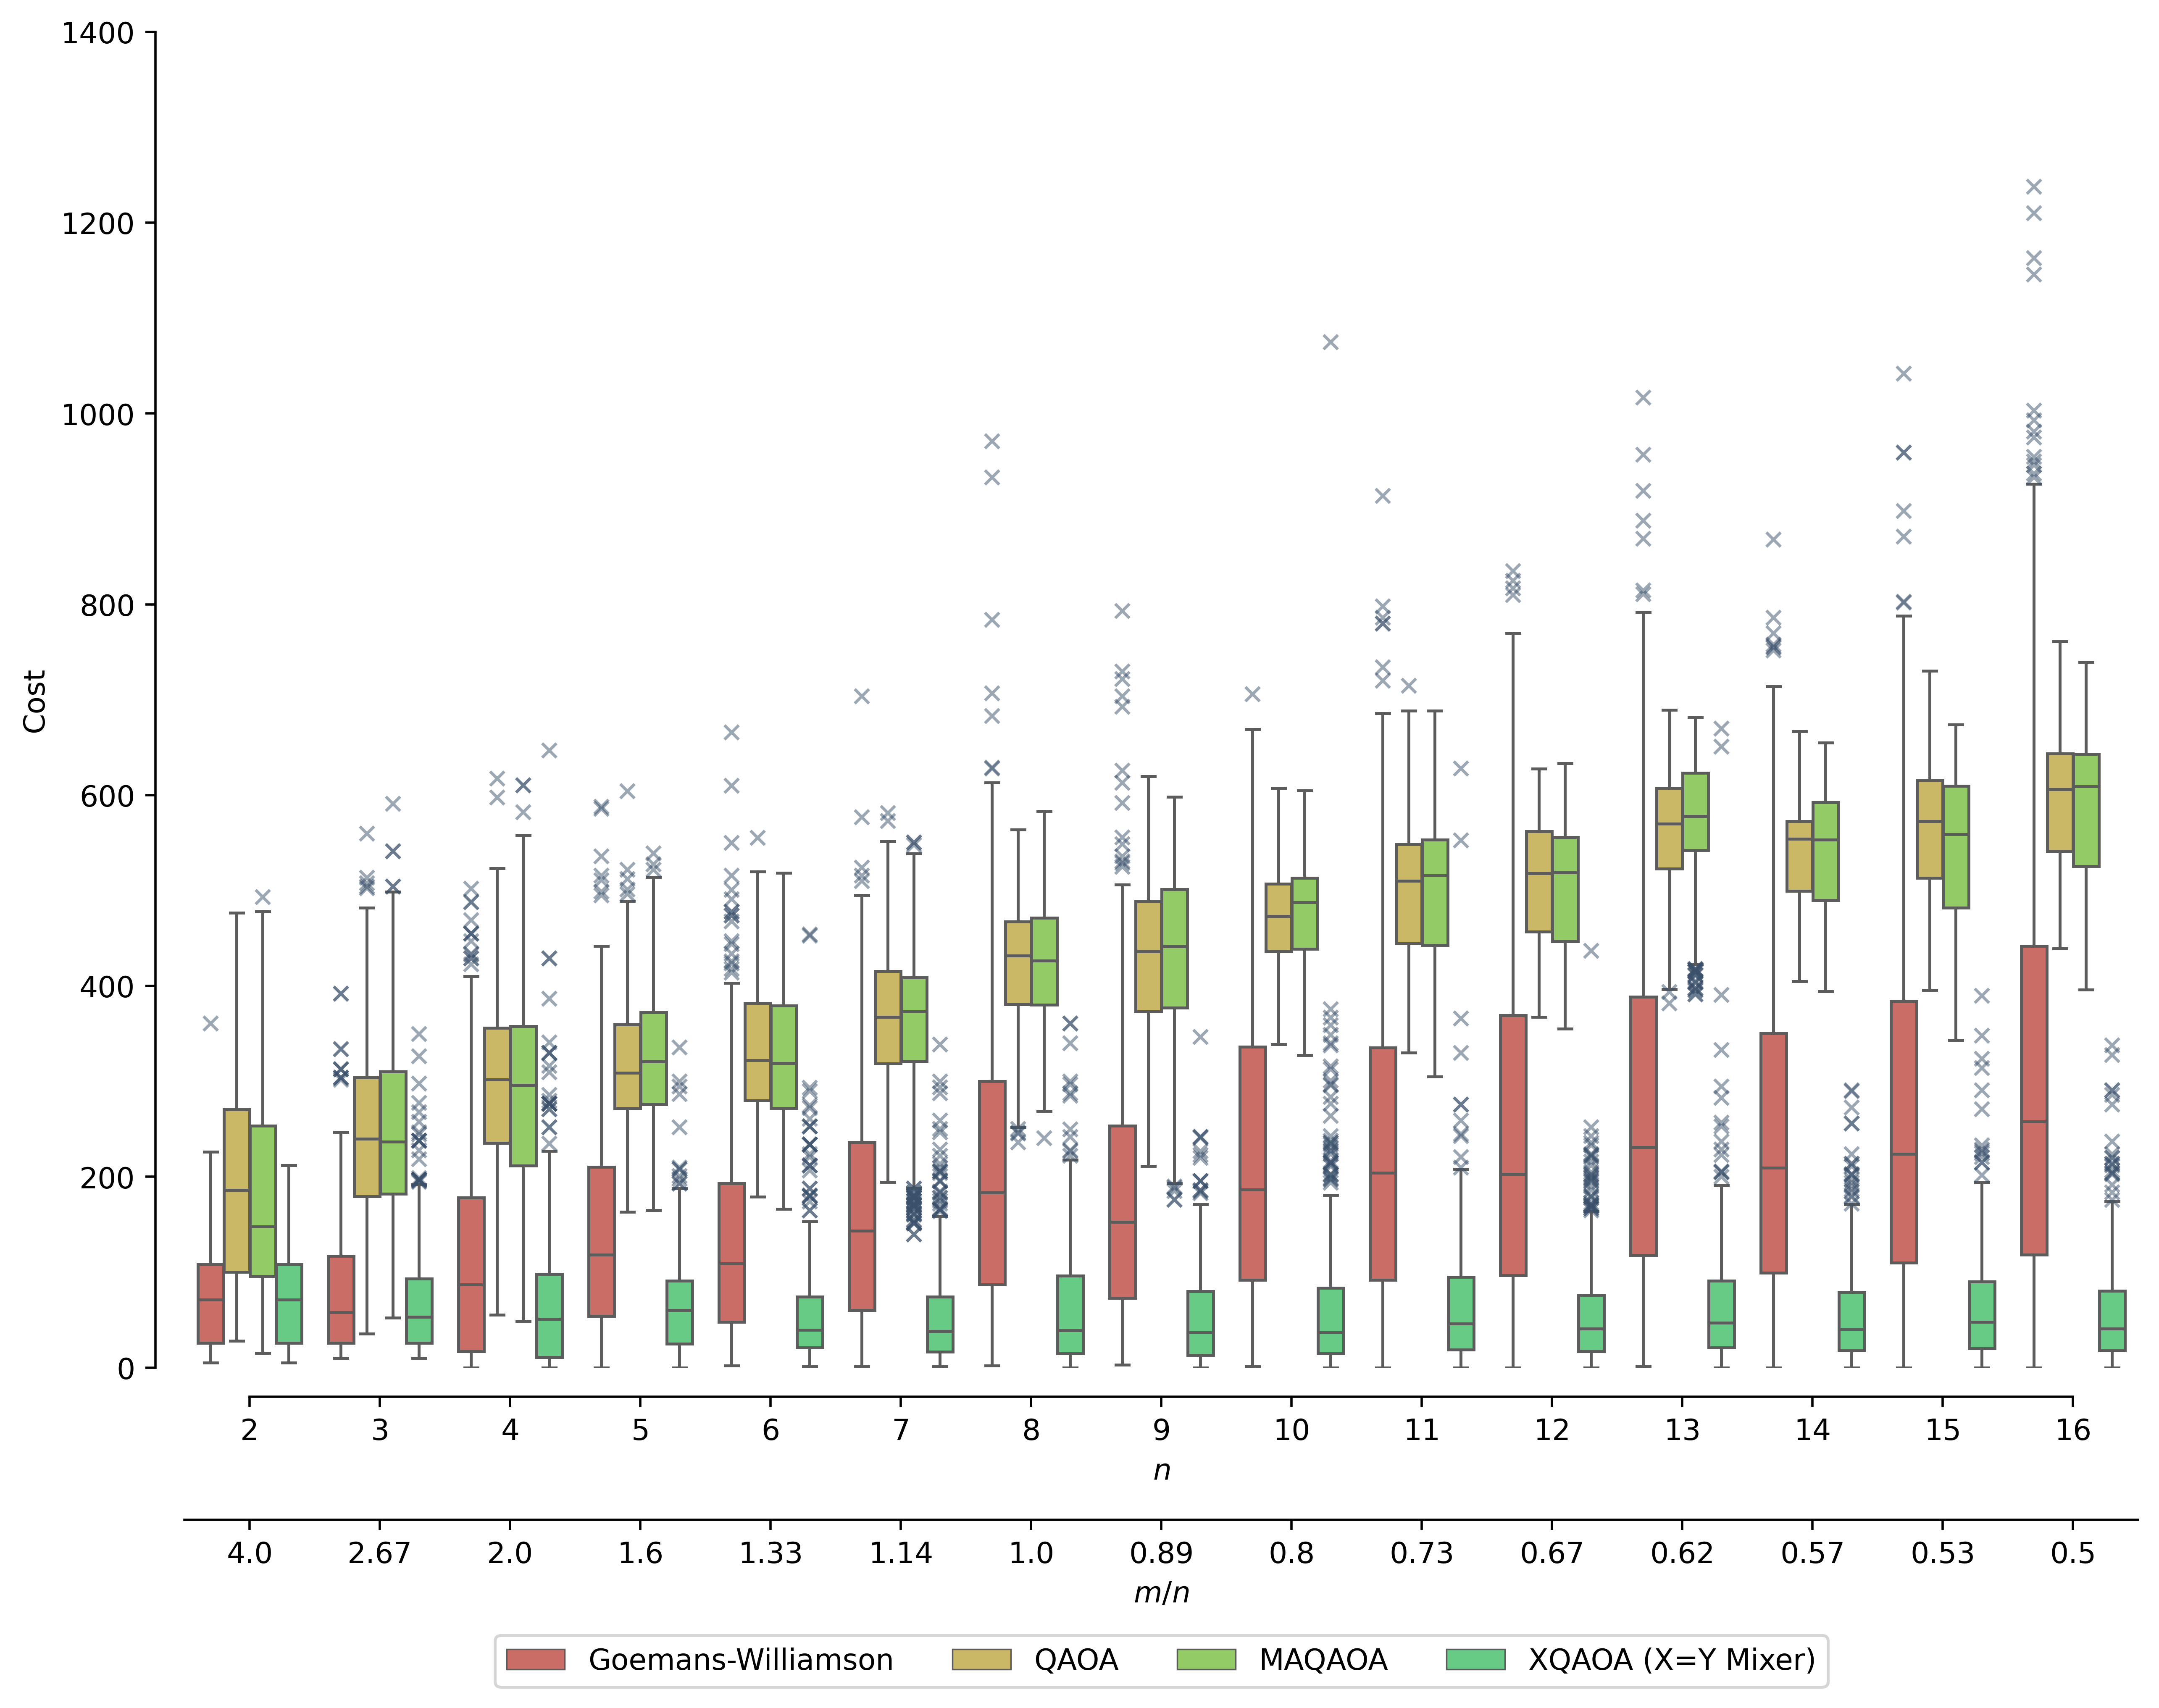
\includegraphics[width=0.48\textwidth]{"../figures/fixed_m_normal.png"}
    \caption{Box plots for problem instances with fixed $m=8$ on a linear scale.}
    \label{fig:fixed_m_normal}
\end{figure}
\subsection{Phase Transition}
The \emph{phase transition} for partitioning problems refers to the transition from problems with high multiplicity of optimal partitions to problems requiring an exhaustive traversal of all possible combinations to guarantee an exact result \cite{hayes2002computing,mertens1998phase}. From Equations 14 and 15 of \cite{mertens1998phase}, for partitioning problems of size $n=10$, the phase transition is $\kappa = 0.88$. As mentioned earlier, the problem ratio $m/n$ was not a good indicator of hardness for the non-classical heuristics, however classical heuristics reflected this phase transition.